\documentclass{article}

\usepackage{amsmath}
\usepackage{graphicx}

\graphicspath{ {python/} }


\setlength{\parindent}{0cm}
\title{PHY 375 - Problem Set 5}

\author{Samuel Barton}

\date{\today}

\begin{document}
	
	\maketitle
	
	\section*{Problem 1}
	
	Let us consider light travelling through air ($n_{\mathrm{air}} = 1.00$)  hitting a glass surface ($n_{\mathrm{glass}} = 1.60$) with an incident angle
	$\theta_i = 30^{\circ}$. 
	
	\subsection*{Part a}
	
	We are now to calculate the reflection and transmission coefficients for both p-polarized and s-polarized light.
	\\
	\\
	First we have the equations for the reflection coefficients
	
	\begin{equation} \label{r_par}
		\mathrm{r}_\parallel = \dfrac{\tan (\theta_i - \theta_t)}{\tan (\theta_i + \theta_t)}
	\end{equation}
	
	\begin{equation} \label{r_per}
		\mathrm{r}_\bot = -\dfrac{\sin (\theta_i - \theta_t)}{\sin (\theta_i + \theta_t)}
	\end{equation}
	\\
	Then we have the equations for the transmission coeffiients
	
	\begin{equation} \label{t_par}
		\mathrm{t}_\parallel = \dfrac{2\sin\theta_t\cos\theta_i}{\sin(\theta_i + \theta_t)}
	\end{equation}
	
	\begin{equation} \label{t_per}
		\mathrm{t}_\bot = \dfrac{2\sin\theta_t\cos\theta_i}{\sin(\theta_i + \theta_t)\cos(\theta_i - \theta_t)}
	\end{equation}
	\\
	Using these four equations we can now calculate all the values for both types of light incident on the glass. Before we continue though, we need
	to calculate the value of $\theta_t$. We can find this easily enough using Snell's Law
	\begin{equation*}
		n_i \sin \theta_i = n_t \sin \theta_t \; \implies 
		\; \sin \theta_t = \dfrac{n_i \sin\theta_i}{n_t} \; \implies 
		\; \theta_t = \sin^{-1}\Big(\dfrac{n_i \sin\theta_i}{n_t}\Big)
	\end{equation*}
	
	If we insert the known values, namely $n_i$, $n_t$, and $\theta_i$ we can calculate $\theta_t$.
	\begin{equation*}
		\theta_t = \sin^{-1}\Big(\dfrac{\sin (30^\circ)}{1.60}\Big) = 18.2^\circ
	\end{equation*}
	Now that we have a value for $\theta_t$ we can now calculate the four values for the reflection and transmission coefficients. First we'll 
	consider the two values for p-polarized light using equations \ref{r_par} and \ref{t_par}. 
	
	\begin{equation*}
		\mathrm{r}_\parallel = \dfrac{\tan (30^\circ - 18.2^\circ)}{\tan (30^\circ + 18.2^\circ)} = 
		\dfrac{\tan (11.8^\circ)}{\tan (48.2^\circ)} = \dfrac{0.209}{1.118} = 0.187
	\end{equation*}
	and
	\begin{equation*}
		\mathrm{t}_\parallel = \dfrac{2\sin(18.2^\circ)\cos(30^\circ)}{\sin(30^\circ + 18.2^\circ)} =
		\dfrac{2\sin(18.2^\circ)\cos(30^\circ)}{\sin(48.2^\circ)} = \dfrac{2 \times 0.312 \times 0.866}{0.745} = 0.725 
	\end{equation*}
	\\
	Now on to the s-polarized light where we'll use equations \ref{r_per} and \ref{t_per}
	\begin{equation*}
		\mathrm{r}_\bot = -\dfrac{\sin (30^\circ - 18.2^\circ)}{\sin (30^\circ + 18.2^\circ)} = 
		-\dfrac{\sin (11.8^\circ)}{\sin (48.2^\circ)} = -\dfrac{0.204}{0.745} = -0.274 
	\end{equation*}
	and
	\begin{equation*}
		\mathrm{t}_\bot = \dfrac{2\sin18.2^\circ\cos30^\circ}{\sin(30^\circ + 18.2^\circ)\cos(30^\circ - 18.2^\circ)} = 
		\dfrac{2\sin18.2^\circ\cos30^\circ}{\sin(48.2^\circ)\cos(11.8^\circ)} = 
		\dfrac{2 \times 0.312 \times 0.866}{0.745 \times 0.979} = 0.741
	\end{equation*}
	
	This gives us the following four values
	$$ \mathrm{r}_\parallel = 0.187 $$
	$$ \mathrm{t}_\parallel = 0.725 $$
	$$ \mathrm{r}_\bot = -0.274 $$
	$$ \mathrm{t}_\bot = 0.741 $$

	\pagebreak
	\subsection*{Part b}
	
	Now let us caluclate the Transmittance and Reflectance for the four values given in part a. Hecht defines the Reflectance and Transmittance of
	light as follows. The reflectance R is
	
	\begin{equation*}
		\mathrm{R} = \dfrac{\mathrm{I}_iA\cos\theta_i}{\mathrm{I}_rA\cos\theta_r} = 
		\dfrac{\mathrm{I}_i}{\mathrm{I}_r} = \Big(\dfrac{\mathrm{E}_{0i}}{\mathrm{E}_{0r}}\Big)^2 = r^2
	\end{equation*}
	\\
	Thus $ \mathrm{R}_\bot = \mathrm{r}_\bot^2$ and $ \mathrm{R}_\parallel = \mathrm{r}_\parallel^2$ which means that the calculation for these
	values in our case is trivial.
	$$ \mathrm{R}_\bot = (-0.274)^2 = 0.075 $$
	$$ \mathrm{R}_\parallel = 0.187^2 = 0.035 $$

	Next we consider the values for the Transmittance T of the light (assuming $\mu_i = \mu_t = \mu_0$):
	
	\begin{equation*}
		\mathrm{T} = \dfrac{n_t\cos\theta_t}{n_i\cos\theta_i}\Big(\dfrac{\mathrm{E}_{0t}}{\mathrm{E}_{0i}}\Big)^2 = 
		\Big(\dfrac{n_t\cos\theta_t}{n_i\cos\theta_i}\Big)t^2
	\end{equation*}

	This givs us the formula to calculate both $\mathrm{T}_\bot$ and $\mathrm{T}_\parallel$. 
	\\
	\\
	First we'll calculat $\mathrm{T}_\bot$.
	
	\begin{equation*}
		\mathrm{T}_\bot = \Big(\dfrac{1.60\cos(18.2^\circ)}{\cos(30^\circ)}\Big)t_\bot^2 = 
		\Big(\dfrac{1.60 \times 0.949}{0.866}\Big)0.741^2 = 0.964
	\end{equation*}
	\\
	and finaly, we'll calculate $\mathrm{T}_\parallel$.
	
	\begin{equation*}
		\mathrm{T}_\parallel = \Big(\dfrac{1.60\cos(18.2^\circ)}{\cos(30^\circ)}\Big)t_\parallel^2 = 
		\Big(\dfrac{1.60 \times 0.949}{0.866}\Big)0.725^2 = 0.526
	\end{equation*}
	\\
	This gives us the values for $\mathrm{T}_\bot$ and $\mathrm{T}_\parallel$. 
	$$ \mathrm{T}_\bot = 0.964 $$
	$$ \mathrm{T}_\parallel = 0.526 $$

	\pagebreak
	
	\section*{Problem 2}
	
	Let us consider the Fresnel equation for the reflective coefficient for perpendicular light
	
	\begin{equation} \label{r-per}
		\mathrm{r}_{\bot} = 
		\dfrac{n_i \cos \theta_i - n_t \cos \theta_t}{n_i \cos \theta_i + n_t \cos \theta_t}
	\end{equation}
	\\
	From Snell's Law we know that $n_i \sin \theta_i = n_t \sin \theta_t$. Now if we multiply equation 
	\ref{r-per} by $ \frac{n_i \sin \theta_i}{n_i \sin \theta_i} $, which we can do since it is just a fancy 
	reprisentation of 1, we can get both the numerator and denominator in a more useful form. 
	
	\begin{equation} \label{r-per-2}
		\mathrm{r}_{\bot} = \dfrac{n_i \sin \theta_i}{n_i \sin \theta_i} \times \Big(
		\dfrac{n_i \cos \theta_i - n_t \cos \theta_t}{n_i \cos \theta_i + n_t \cos \theta_t} \Big) = 
		\dfrac{n^2_i \sin \theta_i \cos \theta_i - n_i n_t \sin \theta_i \cos \theta_t}
		{n^2_i \sin \theta_i \cos \theta_i + n_i n_t \sin \theta_i \cos \theta_t}
	\end{equation}
	\\
	Now, since $n_i \sin \theta_i = n_t \sin \theta_t$ we can replace $n_i \sin \theta_i$ with $n_t \sin \theta_t$ in equation \ref{r-per-2} to get 
	
	\begin{equation} \label{r-per-3}
		\mathrm{r}_{\bot} = 
		\dfrac{n_i n_t \sin \theta_t \cos \theta_i - n_i n_t \sin \theta_i \cos \theta_t}
		{n_i n_t \sin \theta_t \cos \theta_i + n_i n_t \sin \theta_i \cos \theta_t}
	\end{equation}
	\\
	If we use the trigonometric identity that says $\sin(a \pm b) = \sin a \cos b \pm \cos a \sin b$ we can see
	that equaiton \ref{r-per-3} will become 
	
	\begin{equation} \label{r-per-4}
		\mathrm{r}_{\bot} = 
		\dfrac{\sin(\theta_t - \theta_i)}{\sin(\theta_t + \theta_i)}
	\end{equation}
	\\
	Since addition is reflexive, aka $a + b = b + a$, and $\sin(-\theta) = - \sin{\theta}$ we can rewrite 
	equation \ref{r-per-4} in the desired form of 
	
	\begin{equation*}
		\mathrm{r}_{\bot} = 
		- \,\dfrac{\sin(\theta_i - \theta_t)}{\sin(\theta_i + \theta_t)}
	\end{equation*}
	
	\pagebreak
	\section*{Problem 3}
	
	Let us consider what happens to $r_\parallel$ as $\theta_i$ goes from $0^\circ$ to $90^\circ$ for two ases, $n_i = 1$ and $n_t = 1.33$ and the 
	opposite. These two cases are displayed in the following two figures.
	
	\begin{figure}[!h]
		\centering
			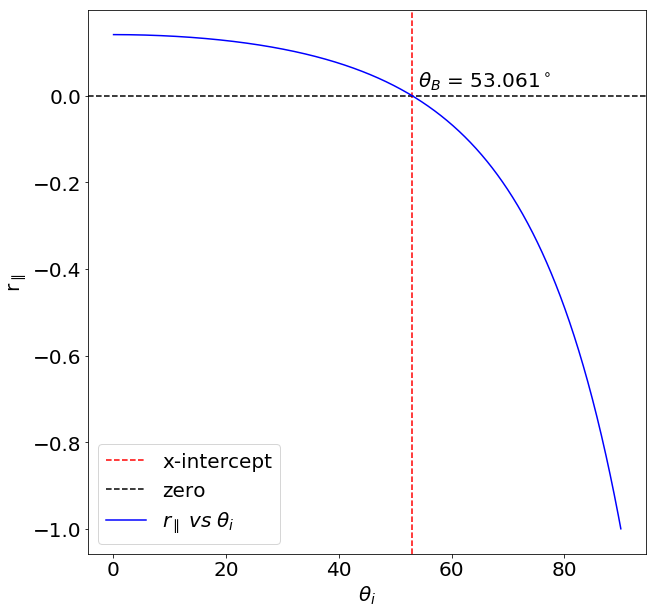
\includegraphics[width=0.75\textwidth]{r-par-1.png}
			\caption{Plot of $r_\parallel$ versus $\theta_i$ where $n_i > n_t$.}
	\end{figure}

	The above figure gives the plot we were looking for. Both it and the plot on the next page were calculated using python. As shown on the plot
	Brewster's Angle for the case where $n_i > n_t$ is $\theta_{brewster} = 53.1^\circ$.

	\begin{figure}[!t]
		\centering
			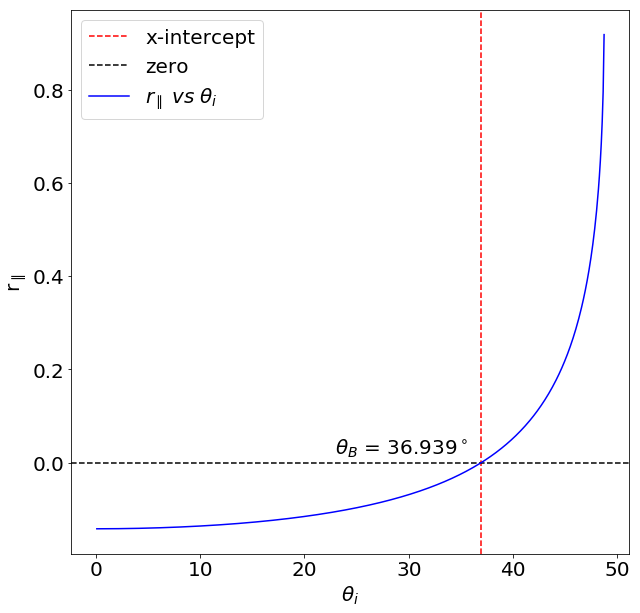
\includegraphics[width=0.75\textwidth]{r-par-2.png}
			\caption{Plot of $r_\parallel$ versus $\theta_i$ where $n_i < n_t$.}
	\end{figure}
	
	\pagebreak
	This figure shows that Brewster's Angle for the case $n_i < n_t$ is $\theta_{brewster} = 36.9^\circ$.
	These two plots give us the information we needed in order to solve Problem 3.
	
	\pagebreak
	\section*{Problem 4}
	
	
	
\end{document}